% SSU Data Dash 2026: team report. Compile from this folder (Overleaf: upload the whole
% repository as a zip). `python run.py report` writes the results table; the other figures come
% from r/slide_figures.R and r/slide_figures_matplotlib.py (see README).
% Keep the report to 4 pages, not counting the outside-data table and the appendix.
\documentclass[11pt]{article}
\usepackage[margin=2.2cm]{geometry}
\usepackage{graphicx,booktabs,hyperref}
\graphicspath{{../figures/}}
\setlength{\parskip}{4pt}
\setlength{\parindent}{0pt}

% TODO before submitting: team name, everyone's full name, and the video link.
\title{SSU Data Dash 2026: \textit{[Team name]}}
\author{Flora [Last name], Ben Rudin, Hannah [Last name], Caitlin [Last name]}
\date{}

\begin{document}
\maketitle
\vspace{-1.5em}

\noindent\begin{tabular}{@{}ll}
\textbf{Video (YouTube, unlisted is fine):} & \url{https://youtu.be/YOUR-VIDEO} \\
\textbf{Code and submission files (GitHub):} & \url{https://github.com/BenIIVVI/datadashstats} \\
\end{tabular}

\section*{Summary}
We value each home in two parts: what it is worth at an average market level, learned by gradient-boosted
trees from 52 features, and where the market will be in the summer it sells, projected from a monthly price
index. A last step corrects each estimate by how the model has been missing on nearby homes of the same type.
On walk-forward validation (December 2025 to May 2026) the off-market model's typical miss is
\textbf{7.31\%} against 17.7\% for the organisers' simple baseline, and on five summers predicted only from
earlier sales it is 6.6--6.9\% in normal years. Most of the remaining error is home quality the data does
not record, which is why condos (5.5\%) are far easier than houses (8.4--8.7\%).

\section{Data and features}
We train on the 150,000 sales from January 2021 to May 2026 and predict the 3,974 off-market and 4,064
list-aware test homes, which sold June to September 2026. We use every column the test files contain. The
after-sale columns (sale date, days on market, the external AVM) are removed from every home we predict;
days on market from \emph{past} sales is used only to guess when a test home will sell (section 2).

\textbf{Market index.} A ridge regression of log price on community $\times$ type, size, bedrooms,
washrooms, parking and one dummy per sale month. The month coefficients are a monthly market level, net of
what sold: it peaks in March 2022 and is about 25\% lower by December 2025, with a dip from spring into
summer every year. Every training price is \emph{deflated} by its month's level, so the tree model learns
what a home is worth at an average market level and the index alone carries time. Working in logs makes every
effect a percentage, which matches how the score is computed.

\textbf{Features (52 per home).}
(i) The home: size (the midpoint when given as a range, plus a flag), bedrooms, washrooms, parking, garage,
lot frontage, depth and area, type, style, municipality, community, latitude and longitude.
(ii) Same building: earlier sales at the exact coordinates (condos share them; for a house it is a repeat
sale), as a count and an average deflated price per sq ft.
(iii) Nearest sales: the median deflated price per sq ft of the 10 nearest earlier sales of the same type,
times this home's size, and their average distance.
(iv) Listing text: a ridge regression on TF-IDF word and word-pair counts (up to 60,000 terms) predicting how
far a home's price per sq ft sits above its community-and-type average, plus 30 SVD topics. The strongest
words are size cues (``studio'' up, ``spacious'' down), then condition (``needs'' and ``as is'' down,
``renovated'' and ``custom'' up) and some street names.
\textbf{No leakage:} a training sale only sees sales from earlier months, cumulative building statistics
exclude the sale itself, and training rows get out-of-fold text scores.

\section{Models}
\textbf{Off-market.} The target is the deflated log price, with recent sales weighted more (a sale's weight
halves every 12 months). The value is the average of four histogram gradient-boosting models
(scikit-learn): two with 2,000 trees at learning rate 0.025 and two with 800 trees at 0.05, all with
leaves of at least 20 sales and 30\% of features tried at each split, each with its own seed. Boosting starts
every home at the average and adds small trees, each fitted to the errors still left; before the local fix,
one tree on its own misses by 11.1\% on the 2024 summer and the four-model average by 6.85\%.
The \emph{market level} for a test home averages the projected index over its likely sale dates: its listing
date plus 100 typical times on market from past sales, kept only if inside June--September. Months past May
are projected as the last level plus the median change for that calendar month in earlier years, so one
unusual year cannot drag the projection.
The \emph{local fix}: five-fold out-of-fold predictions give an honest miss for every training sale. For a
new home we average the misses of its 5, 10, 20 and 40 nearest earlier sales of the same type and combine
the four averages with weights fitted by ridge regression per property type (each sale left out of its own
average); detached houses lean on the widest ring. The prediction is
$\exp(\textrm{value} + \textrm{market level} + \textrm{local fix})$: the three log parts multiply in dollars.
For example, one detached house in the 2024 backtest: \$898,771 $\times$ 0.990 (June market) $\times$ 1.121
(its area sells above the model's guesses) $=$ \$997,309; it sold for \$994,600.

\textbf{List-aware.} Here the target is log(sale / list price), net of a monthly sale-to-list level that is
projected into the summer the same way (at half the seasonal change, which has shrunk every year). Inputs are
the off-market features plus the log list price, the gap between the list price and the off-market
out-of-fold value, the days already listed at the prediction date and the recent sale-to-list level;
training rows simulate predictions made 0--3 months before the sale, as in the test. The off-market value
is what makes the list price informative: an overpriced listing sells further below its list.

\section{Validation}
\textbf{Walk-forward} (the numbers we report): each month from December 2025 to May 2026 is predicted by
models trained only on sales before it, six full refits. \textbf{Summer backtests} copy the real test: train
on sales before June 1, predict June to September. Every modelling choice was made on the 2023 and 2024
summers; 2025 was held back. It was first checked once, and looked at again after the last two changes, so
we treat it as a confirmation rather than a pristine holdout. We also ran 2021 and 2022 with the final model
(not used for any choice). We never used a random split, which would let the model learn from sales after
the ones it predicts.

\section{Results}
\begin{table}[h]
\centering\small
% Written by `python run.py report`. Do not edit by hand: rerun the command instead.
\begin{tabular}{lrccc}
\hline
Track & Homes & MdAPE \% (95\% CI) & MAPE \% (95\% CI) & Median signed error \% \\
\hline
off-market & 10,069 & 7.57 (7.41--7.73) & 9.77 (9.60--9.95) & +1.32 \\
list-aware & 10,069 & 3.85 (3.76--3.94) & 4.92 (4.84--5.00) & -0.09 \\
\hline
\end{tabular}

\caption{Walk-forward validation, December 2025 to May 2026. MdAPE: median absolute percentage error.
MAPE: mean absolute percentage error. Brackets: bootstrap 95\% interval (homes treated as independent).}
\end{table}
\begin{table}[h]
\centering\small
\begin{tabular}{lccccc}
\toprule
Summer (train before June 1) & 2021 & 2022 & 2023 & 2024 & 2025 (held back) \\
\midrule
Off-market MdAPE / MAPE \% & 7.56 / 10.07 & 8.30 / 11.60 & 6.62 / 8.88 & 6.64 / 8.96 & 6.84 / 9.08 \\
Off-market median signed error \% & +0.4 & +5.1 & +0.9 & +1.5 & +0.9 \\
List-aware MdAPE / MAPE \% & & & 4.55 / 5.65 & 4.27 / 5.34 & 3.85 / 4.88 \\
\bottomrule
\end{tabular}
\caption{Summer backtests. 2021 had five months of training data; 2022 is the year prices fell fast.}
\end{table}

Off-market, the typical miss falls from 17.7\% (simple baseline) and 20.8\% (starter, 10 nearest sales) to
7.31\%; list-aware falls from 7.3\% (the list price) to 3.81\%. The validation figure is higher than the
summers because March and April 2026 were hard months (7.9\% and 7.7\%) as prices rose quickly that spring;
the other four months were 6.8--7.2\%. The hidden test is a summer, so we expect about 6.7--7.0\% off-market
unless the summer market turns sharply (see 2022). Across all 54,991 out-of-sample predictions (figure 1),
64\% land within 10\% of the sale price and 89\% within 20\%. Tuning the trees and learning the local-fix
weights cut the typical miss by about 0.2 points on the development summers.

\begin{figure}[h]
\centering
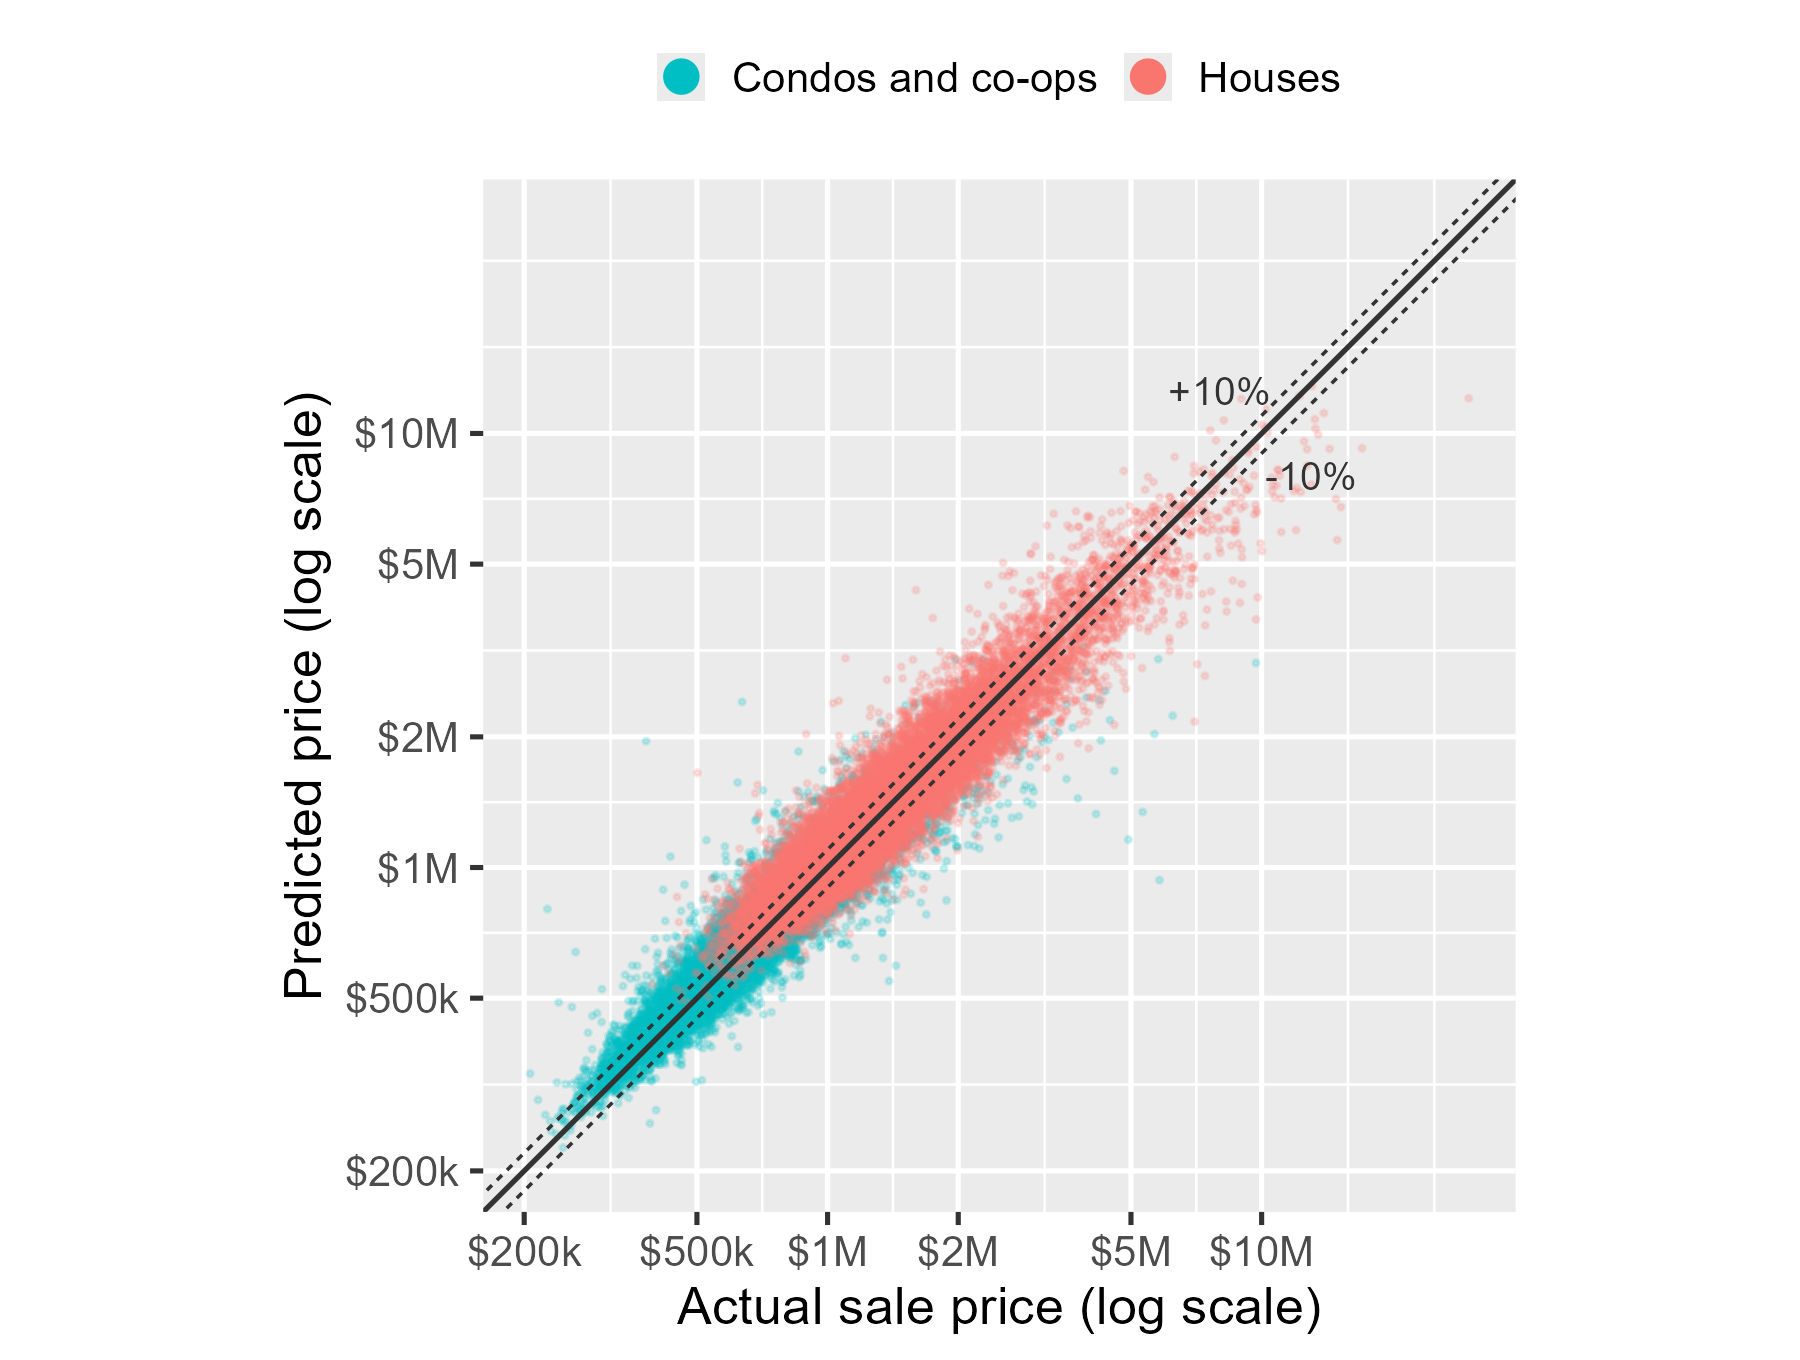
\includegraphics[width=0.48\linewidth]{slides/predactual.png}
\caption{Predicted against actual price for every out-of-sample prediction (five summers and the
walk-forward months), log scales. Solid: perfect; dotted: $\pm$10\%.}
\end{figure}

\section{Where the model fails}
\begin{figure}[h]
\centering
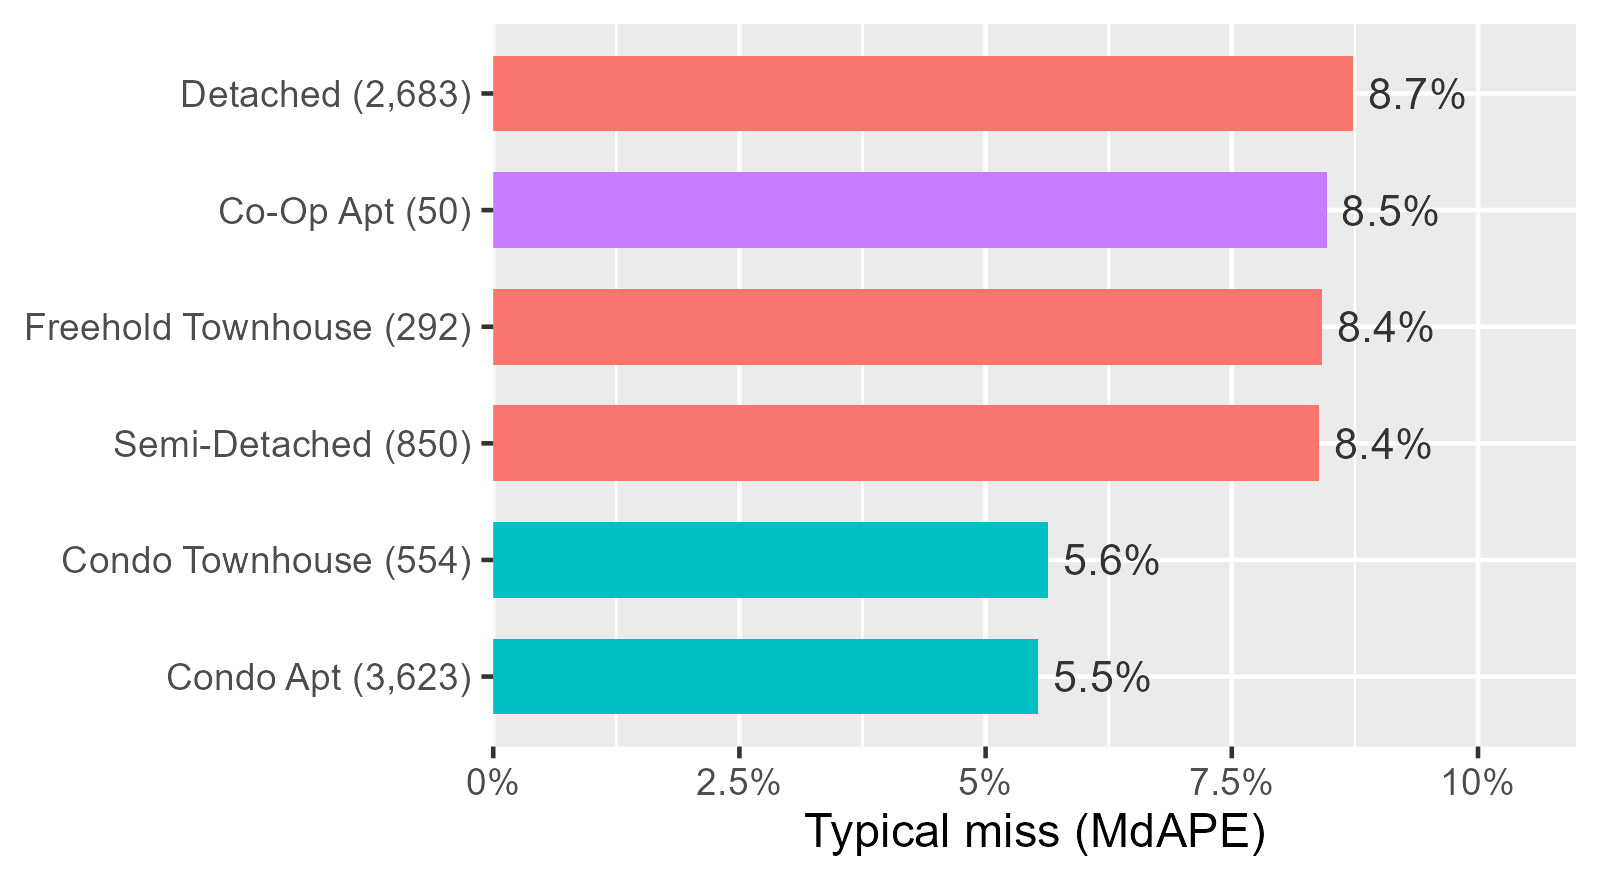
\includegraphics[width=0.49\linewidth]{slides/failures_type.png}\hfill
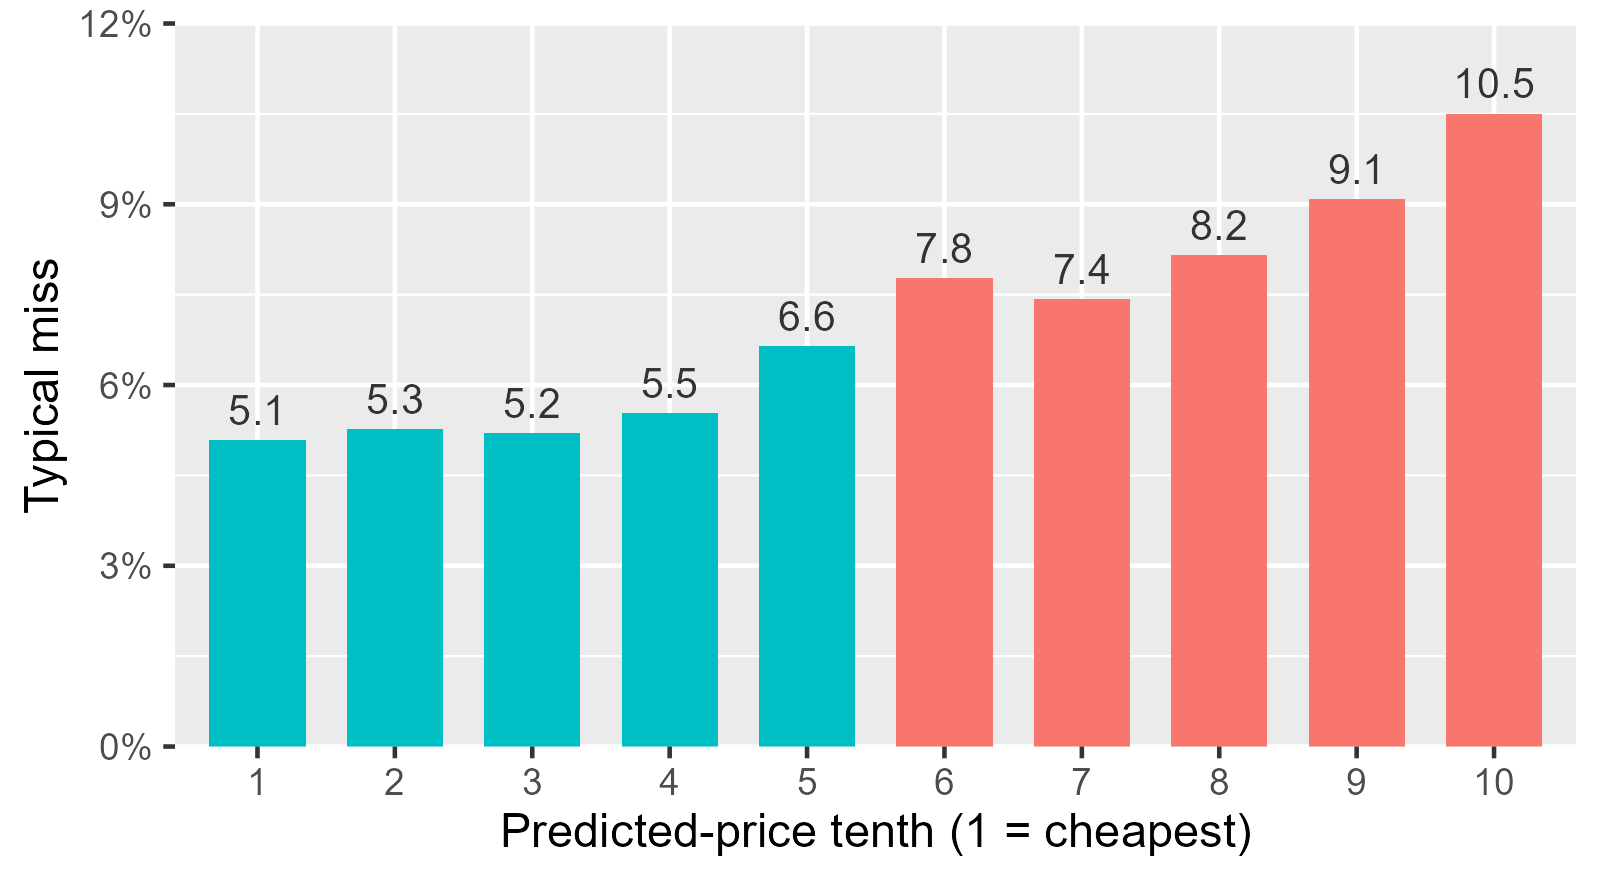
\includegraphics[width=0.49\linewidth]{slides/failures_decile.png}
\caption{Typical miss on the 2025 summer by property type (homes in brackets) and by tenth of predicted
price.}
\end{figure}
\textbf{Type.} Condos miss by about 5.5\%, houses by 8.4--8.7\%. Condos in one building are near-copies, so
building history pins them down; two houses with the same size, rooms and street can differ in age,
renovation, lot and finish, none of which the data records. \textbf{Price.} The cheapest tenth misses by
5.1\%, the dearest by 10.5\%: expensive homes are rarer, more varied and mostly houses.
\textbf{Neighbourhood.} Across the 97 communities with at least 40 sales in 2025, the typical miss ranges
from 3.9\% to 13.5\% (middle half 6.1--8.0\%). It is worse where more sales are houses (correlation 0.39)
and where prices are higher (0.43). The worst are house-heavy areas such as Lindencliffe (13.5\%, 73\% houses,
estimates 4.9\% high) and Hazelfield (10.3\%, 93\% houses, median \$2.27M, 7.4\% low); the best are condo
areas such as Cedarglen (3.9\%). \textbf{Time.} Estimates lean about 2\% high in July and August, when the
summer dip runs deeper than the projection, and 5\% high in 2022, when prices fell after the spring peak.

\textbf{Honest uncertainty.} An 80\% range for each estimate, taken from the 10th to 90th percentile of the
2023--24 misses for its property type, covered 79.5\% of the 2025 homes; its typical width is 22.6\% of the
price (roughly $\pm$11\%). The bootstrap intervals in table 1 assume homes are independent; homes sold in the
same month share the same market surprise, so the real uncertainty is somewhat wider.

\section{Limitations}
\textbf{What did not help}, all judged on the 2023 and 2024 summers: separate indexes for houses and
condos (worse: the projection noise outweighed the bias it fixed); a sharper target for the text model (no
change); following community price trends (changes in a community's premium have autocorrelation $-0.41$,
so they reverse rather than persist); blending in a random forest (9.2\% on its own); neighbours matched on
size, or on the exact same layout; separate tree models for houses and condos; a fixed summer bias
correction (the best shift varied from 0 to 1.75\% by year).
\textbf{When not to trust it:} expensive and unusual houses; a summer when the market turns sharply; thin
groups such as co-ops (50 test homes in 2025) and rarely traded communities. The data say nothing about age,
renovation, floor level or condo fees, and those would help most. Next we would try quantile models for
the ranges, and a projection that reacts to the most recent months instead of only past summers.

\section*{Outside data}
\begin{tabular}{lll}
\toprule
Source & URL & Periods covered \\
\midrule
None & & \\
\bottomrule
\end{tabular}

\section*{Reproducing our results}
From a fresh copy of the repository (the data downloads itself on first use):\\
\texttt{pip install -r requirements.txt}\\
\texttt{python run.py backtest \&\& python run.py validate \&\& python run.py report}\\
\texttt{python run.py predict \&\& python run.py check}\\
All seeds are fixed, so these commands rebuild the two submission files exactly. The figures come from
\texttt{python r/slide\_figure\_data.py}, \texttt{Rscript r/slide\_figures.R} and
\texttt{python r/slide\_figures\_matplotlib.py}.

\end{document}
